\documentclass[]{article}
\usepackage[width=150mm,top=30mm,bottom=30mm]{geometry}

\usepackage{graphicx}
\usepackage{hyperref}
\usepackage{float}
\usepackage{listings}
\usepackage{txfonts}  
\usepackage{epstopdf}
\usepackage{textcomp}
\usepackage{mathtools}

\usepackage{tikz}

\newcommand{\shellcmd}[1]{\\\indent\indent\texttt{\footnotesize\$ #1}\\}

\begin{document}

\title{\textbf{Exercise: Dye anchoring to  TiO$_{2}$ AceticAcid}}
\author{\textbf{Technical Chemistry - Lab Course - SommerSemester 2018}}
\date{July 9, 2018}

\maketitle

\begin{figure}
\centering
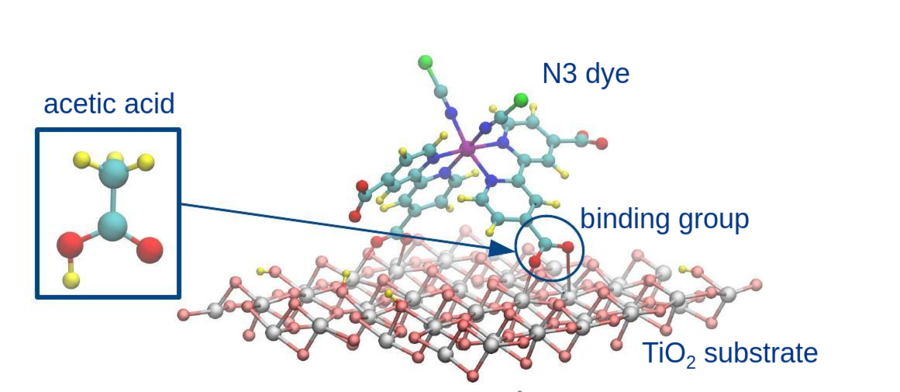
\includegraphics[width=0.80\linewidth]{dye1.png}
\label{fig:dye1}
\end{figure}


\subsection*{Exercise 1:\underline{Visualization of Geometries}}


In this exercise you will compare two possible binding modes of acetic acid to anatase TiO$_{2}$. Acetic acid contains the carboxylic group. It is commonly used in Dye-Sensitized Solar Cells as an anchoring moiety to bind light harvesting dyes to semi-conducting substrates. We will therefore use acetic acid as a model of the more complex dye molecules.
\newline
\newline
\textbf{1.} Download the folder "MaterialsScience" from the path /upb/groups/ak-kuehne/public/share into your home directory. To copy it to your home directory use the following command in your home directory:
\newline
scp -r /upb/groups/ak-kuehne/public/share/MaterialScience .
\newline
\newline
\textbf{2.} In the following exercises try to keep your files and directories organized in a suitable manner. If not, there is a high danger of errors, that may lead to loss of data and your time. One option would be renaming files and creating own folders for each calculation. 
\newline
\newline
Geometries are generally stored in files with the ending ".xyz", while input-files have the ending ".inp" and output-files ".out". An easy way to visualize a geometry is the program VMD. To use VMD, type vmd "name of geometry-file" into the linux terminal. VMD has a wide variety of options for visualization and analysis. In the downloaded directory there is also a pdf-file named "vmd-tutorial" that should help you with handeling vmd over the course of the exercise. The menu can be switched on by typing "menu main on" in the command line. Generally useful ones for this exercise are:
\newline
\newline 
\newpage
To visualize a system:
Graphics $>$ Representations $>$ Draw style $>$ Drawing Method: CPK
To visualize the MO structure in VMD:
Graphics $>$ Representations $>$ Draw style $>$ Drawing Method: Isosurfaces
In Isosurfaces, set Draw to “Wireframe” 
In Isosurfaces, set Isovalue to 0.1, 0.01 …
To visualize the positive and the negative part of an orbital simultaneously, add a second isosurface representation with isovalues -0.1, -0.01, …
To give the two representations different colors, set their “Coloring Method” to “ColorID” and choose different ids. 
\newline
\newline
\textbf{3.} Visualize the geometries mode1.xyz and mode2.xyz from the directory "Exercise1" and familiarize yourself with the system. Render both geometries or make screenshots for your report.  
\newline
\newline
\textbf{4.} Briefly sketch the two binding modes and discuss your findings. The following questions might be helpful in that regard. What is the binding of acetic acid on TiO$_{2}$ an interesting areas of research? Are mode1 and mode2 valid representations of a real system and if why is that the case? Why do we use anatase TiO$_{2}$? What possible binding modes are there and what are their differences. How do mode1 and mode2 compare to that. What is the importance of proton transfer in this system? 
     
\subsection*{Exercise 2:\underline{Bond induced density differences}}

In this part of the exercise we want to compute the electronic density difference induced by the bonding for the first binding mode to analyze its nature. This will be done by using DFT energy calculations. In the directory "Exercise2" there is an input-file "basic.inp". It also includes the files "BASIS-SETS" and "POTENTIALS", that are needed to calculate the energy. Those files and the geometry file have to be linked to the input file. In the input file, there are "empty" brackets, that have to be filled out for each task accordingly.  
\newline
\newline
\textbf{1.} Run an energy calculation for the combined system of mode1. Also run energy calculations for the lone acetic acid molecule and the lone TiO$_{2}$ slab. For that adapt the "basic.inp" and the coordinate file for each of the three runs. 
\newline
\newline
The general structure to start a calculation with cp2k is the following:
\begin{center}
$mpirun -n \ \ 2 \ \ cp2k.popt\ \ "Input-file" \ |\ tee \ \ "Output-file" ,$
\end{center} 
with cp2k.popt being the executable of the program and placeholders for the names of the In- and Output-files. This command runs the calculation in a parallel process with two cores and produces output-files with the ".out" and ".cube" ending (if enabled in the input-file). 
\newline
\newline
\textbf{2.} Please calculate the bond induced electronic density difference. You should do that using the previous 3 energy calculations and the tool cubecruncher, which you also downloaded. To calculate the difference in electronic density through the bonding subtract the lone electron densities of the slab and acetic acid from those in mode1. The electron densities are stored in the generated cube file for each calculation. You can visualize the electron density of each calculation with VMD.
\newline
\newline
The tool "cubecruncher" is avaiable in the folder "MaterialsScience". Open a terminal in the folder "cubecruncher" and type "make". That compiles the executable. Then copy the executable "cubecruncher.x into your working directory. The basic structure of a subtract command is:
\begin{center}
$./cubecrunsher.x \ \ -i \ \ "First.cube" \ \ -subtract\ \ "Second.cube" -o \ \ "Output.cube"$,
\end{center}
where Second.cube's values are subtracted from those in the file First.cube and the results are stored in Output.cube. Please adapt the command according to the filenames you are using. 
\newline
\newline
\newpage
\textbf{3.} Visualize the resulting ".cube"-file with VMD as you have learned before. You will see, that the system is not centered inside your simulation box anymore. You can use cubecruncher again to center your system. The basic command is:
\begin{center}
./cubecruncher.x \ -center geo \ -i \ "Notcentered.cube" \ -o \ "Centered.cube"
\end{center}


Keep in mind to center your system in the simulation box. Use Isosurfaces to visualize the electron density difference and discuss what you can observe. Isosurfaces can be created in the graphics category. Create a new representation for each isosurface. Discuss your results. How do the results fit to your answer in Exercise 1 regarding the type of binding in mode 1? 




\subsection*{Exercise 3:\underline{Bonding energies}}

The binding energy for both binding modes is described as:

\begin{center}
$E_{binding}=\sum E_{products}-\sum  E_{reactants}.$
\end{center}
\newline
\textbf{1.} Calculate the bonding energy for both binding modes. You generally can find the converged energies in the output-file of a calculation. 
\newline
\newline
Calculate all needed energies. For the lone TiO$_{2}$ slab you can use the coordinates from "relaxedslab.xyz", which are in the directory "Exercise3". Why is it not feasible to use all of the energy results from exercise 2.1? For which cases is it possible to use past results and why? Do a geometrical optimization for the relaxed slab. It should converge rather quickly. 
\newline
\newline
\textbf{2.} Report the system energies for both modes, the lone slab and the acid molecule. Which mode is more stable? Discuss your findings and relate them to what you have learned in the previous exercises. 
\newline
\newline

Good luck!








\end{document}


